\begin{frame}{Construcción de diccionario (1/3)}

    \begin{block}{Características}
        \begin{itemize}
            \item Conjunto de 13 imágenes en alta resolución del \emph{dataset MIRFLICKR}
            \item Imágenes sin relación alguna
            \item Tamaños diferentes
        \end{itemize}
    \end{block}

    \begin{figure}[H]
        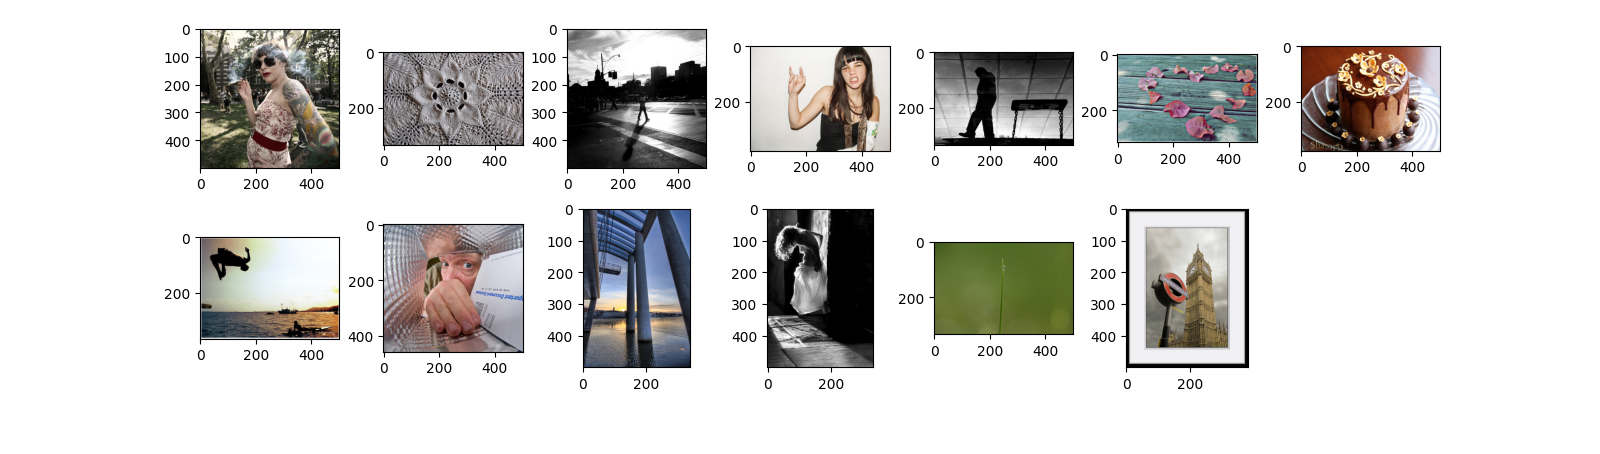
\includegraphics[scale = 0.3]{ fr_dataset.png }
        \centering
        \caption{ \emph{Dataset} utilizado para construcción de diccionario}
        \label{fig:fr_dataset}
    \end{figure}
\end{frame}

\begin{frame}{Construcción de diccionario (2/3)}

    \begin{block}{Requisitos de cada imagen}
        \begin{itemize}
            \item Paridad entre baja y alta resolución
            \item Filtrado pasa-altas
            $\text{img}_f = \text{img} - \text{\emph{cv2.GaussianBlur}}(\cdot)$
            \item Normalizado
            $\text{img}_n = \frac{\text{img}_f-\text{min}(\text{img}_f)}{\text{max}(\text{img}_f)-\text{min}(\text{img}_f)}\cdot 255$
        \end{itemize}
    \end{block}

    \begin{figure}[H]
        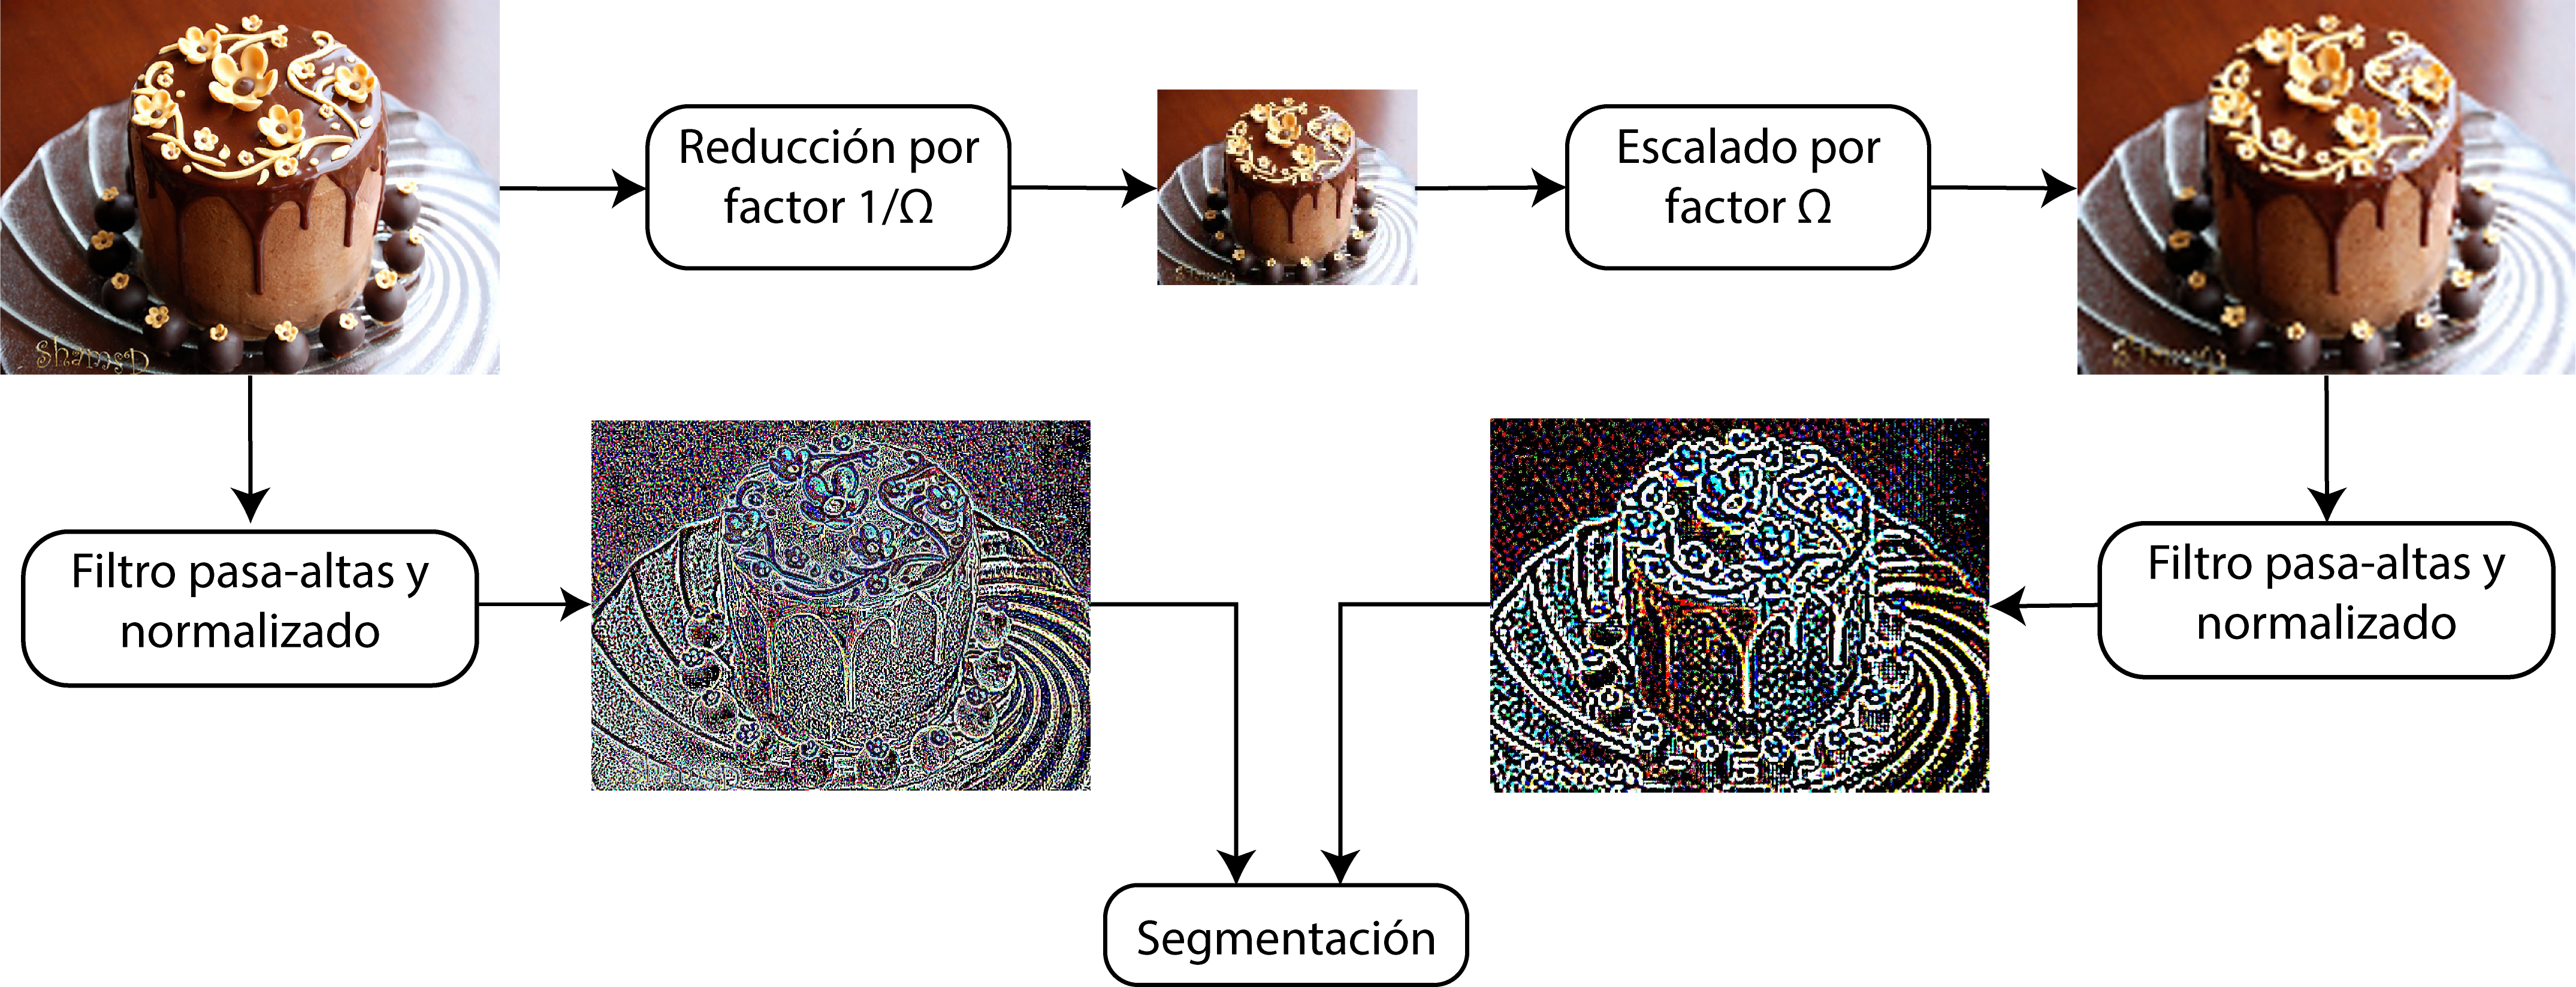
\includegraphics[scale = 0.4]{ fr_prepdic.png }
        \centering
        \caption{Preparación de imágenes mediante algoritmos de interpolación}
        \label{fig:fr_interpolacion}
    \end{figure}
\end{frame}

\begin{frame}{Construcción de diccionario (3/3)}

    El \emph{segmentador} tiene el objetivo de recolectar los parches en alta y baja resolución con 
    dimensiones de $5\times5$ y $7\times7$ respectivamente.

    \begin{figure}[H]
        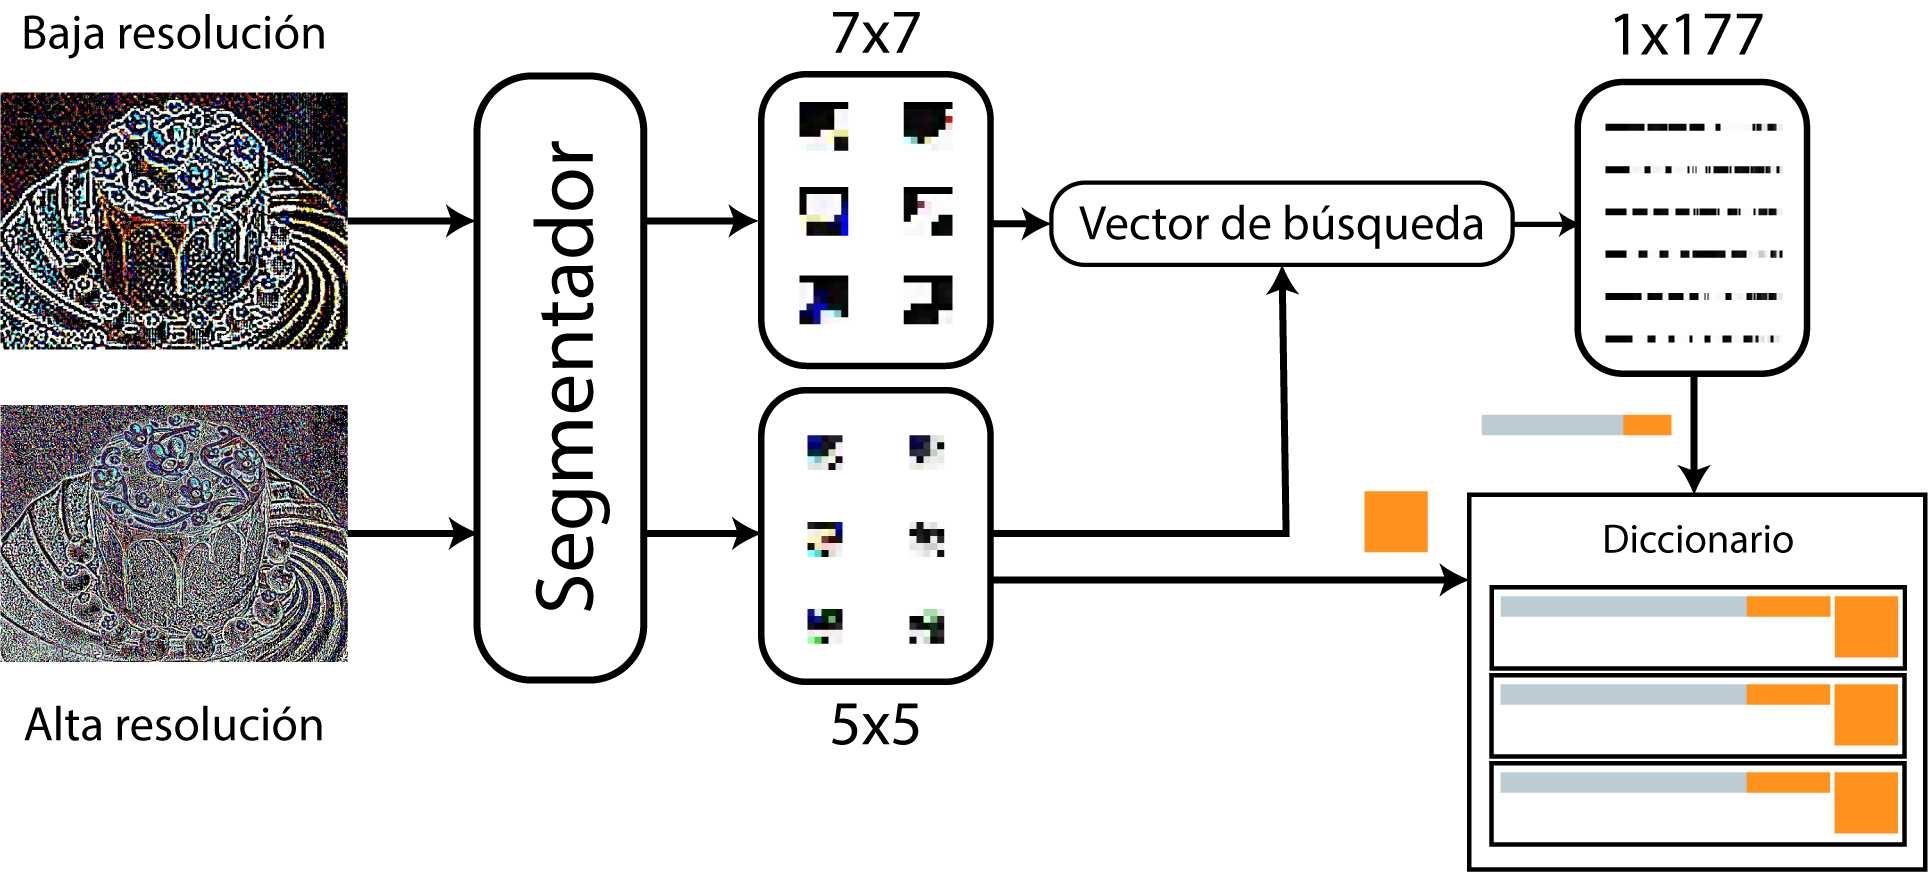
\includegraphics[scale = 0.8]{ fr_segmentado.png }
        \centering
        \caption{ Segmentación y almacenamiento de parches en diccionario }
        \label{fig:fr_segmentador}
    \end{figure}

    Los 154,125 vectores recolectados son almacenados en \emph{diccionario.h5} mediante
    el paquete \emph{h5py}.

\end{frame}

\begin{frame}{Algoritmo de búsqueda (1/2)}

    Utilizando la función \emph{NearestNeighbors} del paquete \emph{sklearn.neighbors},
    la implementación resulta sencilla una vez ordenados todos los vectores en el 
    diccionario. 

    \begin{figure}[H]
        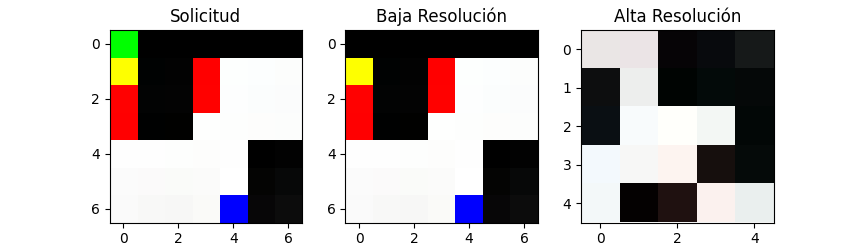
\includegraphics[scale = 0.5]{ fr_vecinos.png }
        \centering
        \caption{ Ejemplo de búsqueda de parches en diccionario}
        \label{fig:fr_vecinos}
    \end{figure}

    Aproximación en 8.9 $s$ utilizando el algoritmo \emph{Ball Tree}. 

\end{frame}

\begin{frame}{Algoritmo de búsqueda (1/2)}

    \begin{block}{Complejidad temporal}
        \begin{itemize}
            \item \emph{Ball Tree} $\to \mathcal{O}[D\,\text{log}|N| ]$
            \item \emph{Fuerza bruta} $\to \mathcal{O}[D\,\text{log}|N| ]$
            \item \emph{KD Tree} $\to \mathcal{O}[D\,\text{log}|N| ] : D < 20$, $\mathcal{O}[D\,N]$
            
            Donde $D$ corresponde a las dimensiones y $N$ el número de elementos.  
        \end{itemize}
    \end{block}

    \begin{table}[H]
        \caption{Tiempos de algoritmo de búsqueda}
        \label{tb:tiempos_snn}
        \centering
        \begin{tabular}{|c|c|}
        \hline
        \textbf{Algoritmo}    & \textbf{Tiempo} {[}s{]} \\ \hline
        Auto         & 9.8            \\ \hline
        Fuerza Bruta & 9.5            \\ \hline
        KD Tree      & 9.5            \\ \hline
        Ball Tree    & 8.9            \\ \hline
        \end{tabular}
    \end{table}

\end{frame}

\begin{frame}{Algoritmo de predicción (1/2)}

    Considerado un escalado con factor  $\Omega=2$ y factor de
    superposición de $\alpha=0.05$.

    \begin{figure}[H]
        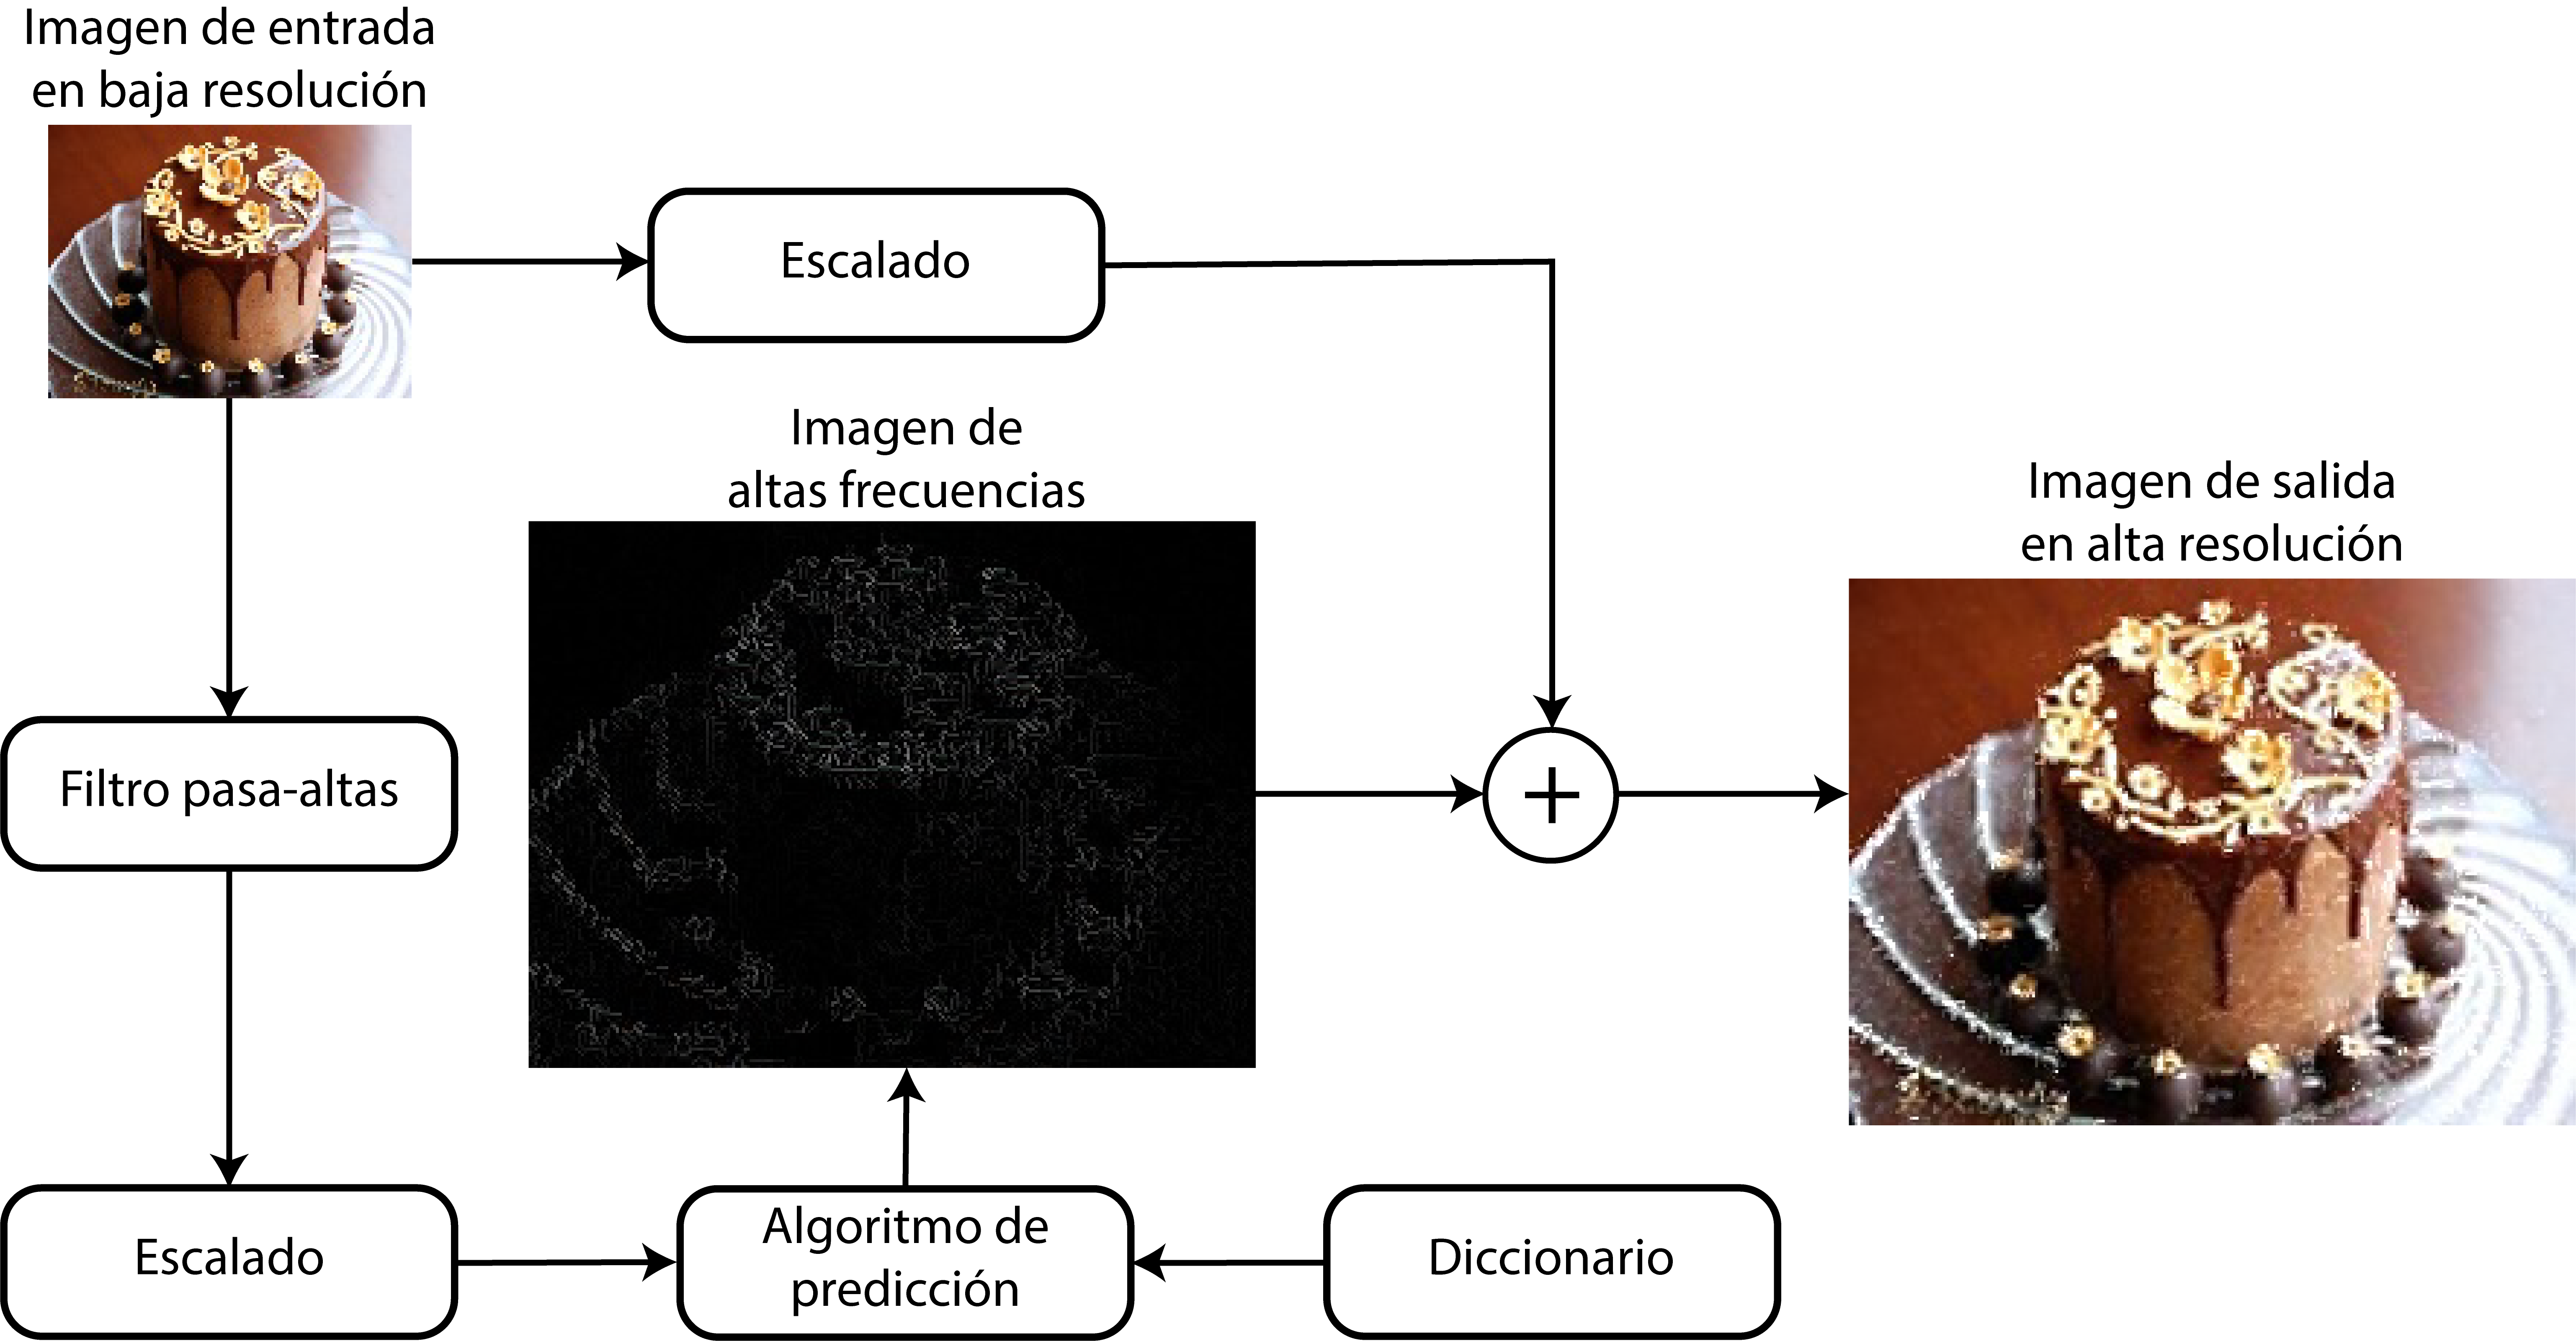
\includegraphics[scale = 0.3]{ fr_proceso.png }
        \centering
        \caption{ Algoritmo de Súper Resolución}
        \label{fig:fr_proceso}
    \end{figure}

\end{frame}

\begin{frame}{Algoritmo de predicción (2/2)}

    El parámetro de superposición permite enfatizar los detalles de
    la imagen de altas frecuencias e indirectamente los detalles de la
    imagen con mejor resolución. Sin embargo, a valores altos tiende a agregarse
    ruido a la imagen y por lo tanto la definición decrece nuevamente.

    \begin{figure}[H]
        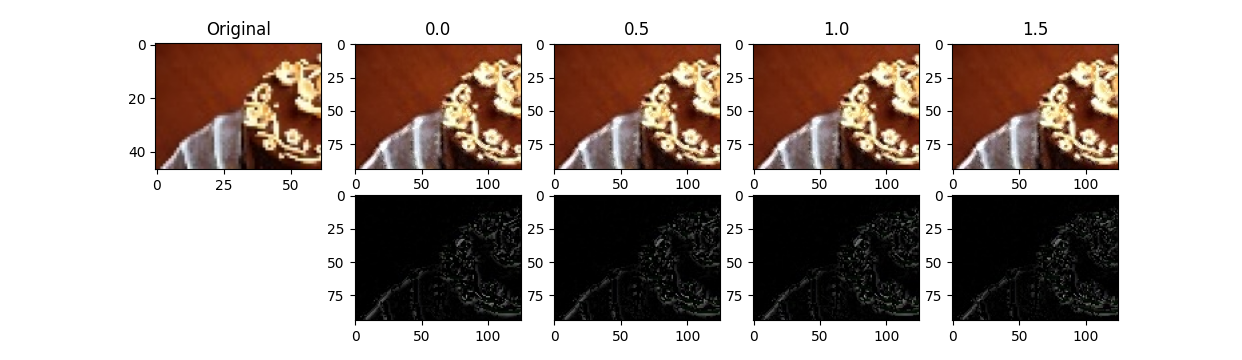
\includegraphics[scale = 0.38]{ fr_alphas.png }
        \centering
        \caption{ Variación en parámetro de superposición $\alpha$ }
        \label{fig:fr_alphas}
    \end{figure}

\end{frame}